\section{Extensional Work}
\subsection{\NP~Hardness}
Bekos et al. proposed a reduction from the \NP-hard problem \texttt{3-CNF-SAT} to a bendless SMOG of maximum degree four by constructing gadgets, which encode a given propositional formula $\varphi$ into an information \grqq flow\grqq~through the gadgets. $\varphi$ is satisfiable if and only if the respective bendless gadget construction preserves planarity.\\
We will extend the proof to graphs with arbitrary degree by creating a tunnel for every edge where all possible realizations with minimum edge complexity are drawn inside.
\begin{assumption} Based on the unit length $l(u)$ between two vertices on the coarse grid, we assume that the size of the vertex boxes are at most $\frac{1}{2}l(u) \times \frac{1}{2}l(u)$.\label{assumption}
\end{assumption}
The box size approximation ensure that a straight-line edge connecting two neighboured vertices on the coarse grid can be drawn. The boxes reach up to $\frac{1}{4}l(u)$ into the edge, ensuring a drawn length of the edge by length minimal $\frac{1}{2}l(u)$. As we already know, the maximal degree $m$ of the graph $G$ yields the granularity of the fine grid causing possible $m$ edges per port regarding a vertex.\\
Regarding the proof for the \NP-hardness of the bendless problem, the main difference between the 4-planar case and the $m$-planar case is the port position of the edge. In the 4-planar case, the position of the straight-line / quarter arc edges is fixed on the center of the port. However, in the $m$-planar case, there are $m$ possible positions on a single port. The main similarity between both cases is the position of the vertices. Because the vertices lie on the coarse grid, the difference in $x$-direction equals the difference in $y$-direction. Furthermore, the $m$ possible quarter arcs inherit the same center of the circles.
\begin{figure}[h]
	\centering
	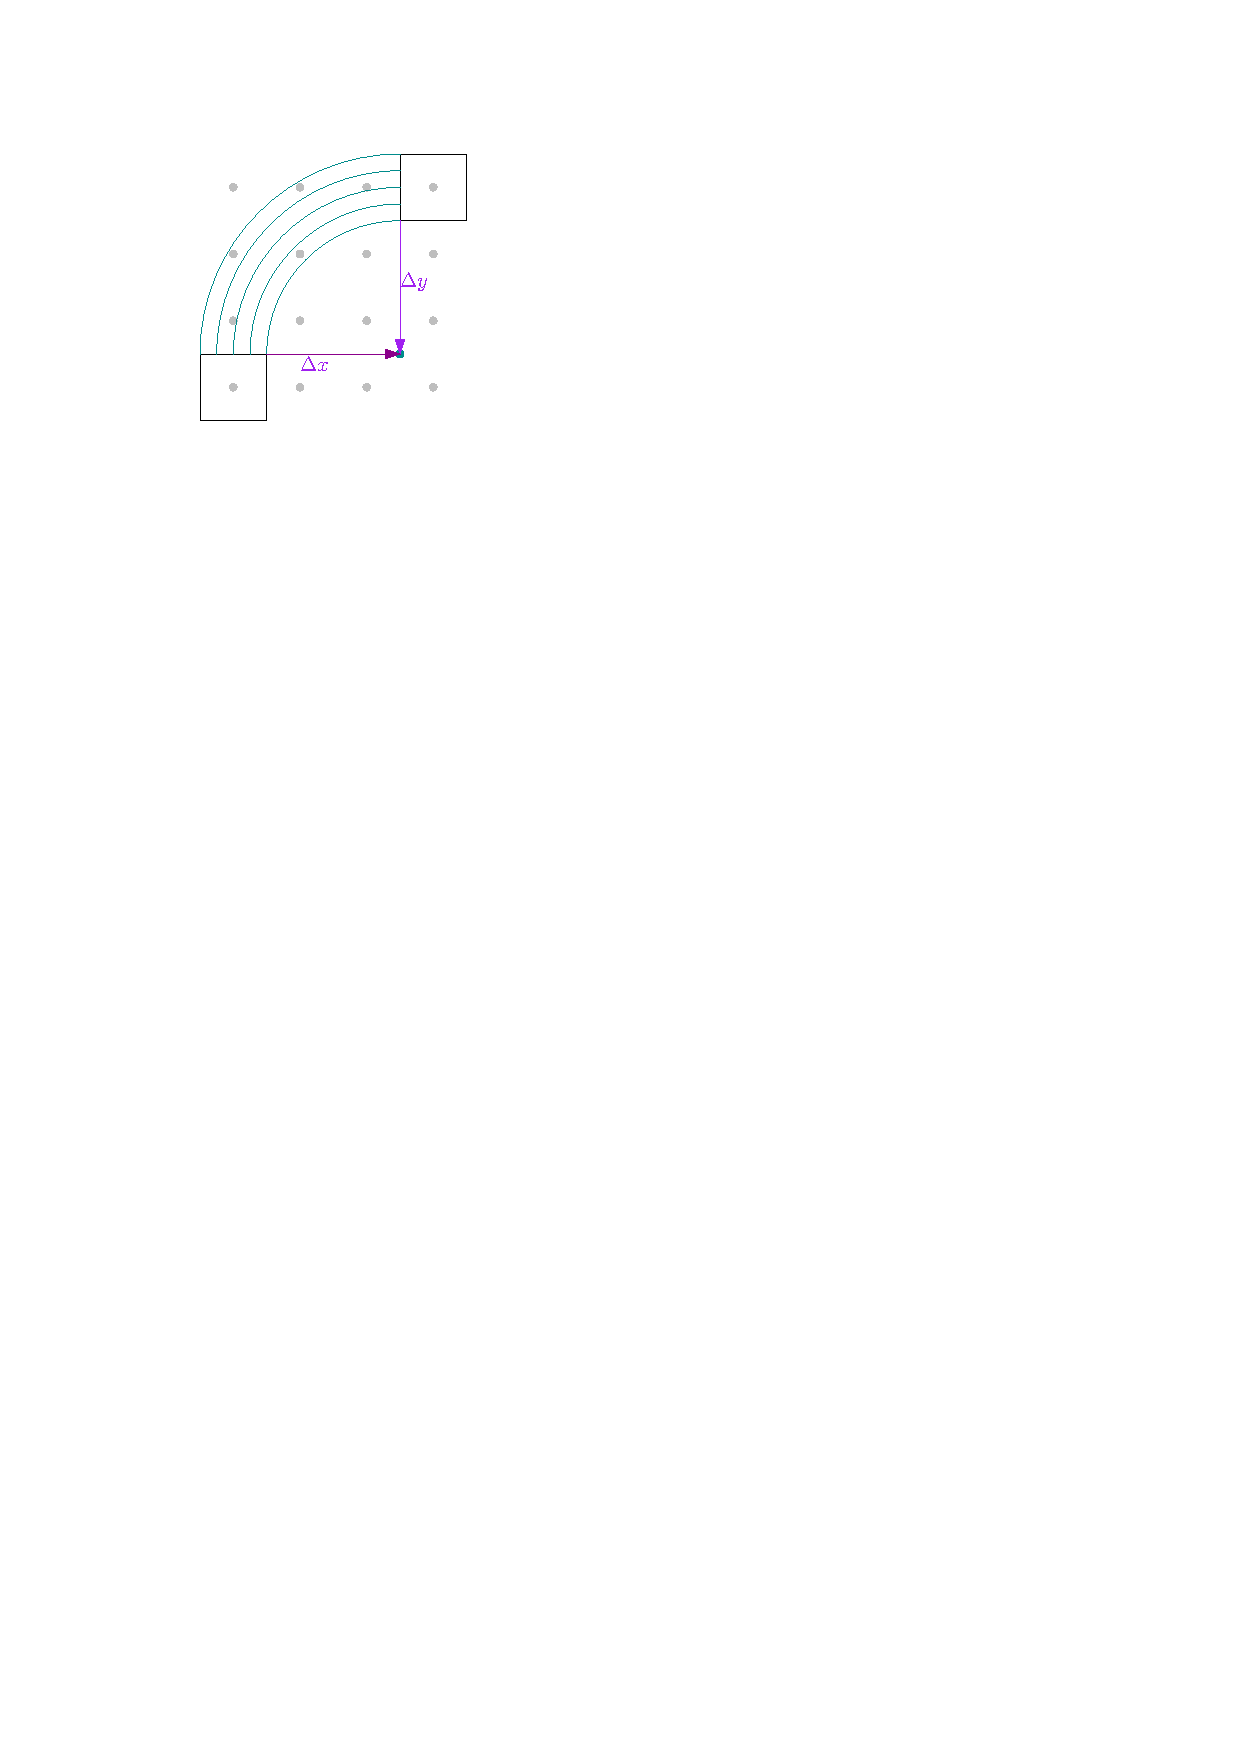
\includegraphics[width=0.3\linewidth,page=1]{includegraphics/NP_center_of_circles.pdf}
	\caption{Multiple possible bendless connections}
	\label{im:mult_poss_connections}
\end{figure}
As depicted in Figure \ref{im:mult_poss_connections}, there are multiple quarter arc connections possible from one vertex to another. They all share the same center (the cyan dot). This also holds for straight line segments between two vertices. This leads to a gauge of the gadgets introduced in the \NP-hardness proof of Theorem \ref{th:NP-hard-4}. We will only illustrate the tunnel for the circular arcs for 	clear visualization. The straight edges between two vertices are interpreted as tunnels.
\begin{theorem}
	Given a planar orthogonal drawing of a graph $G$ of arbitrary degree and a SMOG representation $\mathcal{R}$, it is \NP-hard to decide if it can be smoothened without any bends, preserving $\mathcal{R}$. The \NP-hardness still holds even if $\mathcal{R}$ requires all edges to be drawn as straight-line segments or quarter circular arcs. This is a slight modification of the gadget construction by Theorem \ref{th:NP-hard-4}.\label{th:NP-hard-m} 
\end{theorem}
\begin{proof}
asically, for the \NP-hardness, the reduction from \call{3-CNF-SAT} is very similar to the construction of $\call{R}_\varphi$ of Theorem \ref{th:NP-hard-4}. However, the gadgets vary.
\begin{itemize}
	\item \textit{Variable gadget}\\
	\begin{figure}[h]
		\centering
		\begin{subfigure}{0.4\textwidth}
			\centering
			\includegraphics*[width=0.9\linewidth,page=1]{includegraphics/NP_m_variable_gadget.pdf}
			\caption{\texttt{true} assignment}
		\end{subfigure}
		\begin{subfigure}{0.4\textwidth}
			\centering
			\includegraphics*[width=0.9\linewidth,page=2]{includegraphics/NP_m_variable_gadget.pdf}
			\caption{\texttt{false} assignment}
		\end{subfigure}
		\caption{new variable gadgets}\label{im:m-variable-gadgets}
	\end{figure}
The variable gadgets inherit the multiple arcs from Figure \ref{im:mult_poss_connections} illustrated by the magenta edges. The maximum radius still values $l(u)$ like in the 4-planar case, but the center is shifted to the regarding corner of the vertex box. This is not a problem for the variable gadgets, however the offset of the center implies possible crossings in the parity gadget.
		\item \textit{Parity gadget}\\
		Looking at the parity gadgets, one can see the possible crossings given by the new possible position of the edges.
		\begin{figure}[H]
			\centering
			\begin{subfigure}{0.6\textwidth}
				\centering
				\includegraphics*[width=0.9\linewidth,page=1]{includegraphics/NP_m_parity_gadget.pdf}
				\caption{\texttt{false} assignment}
			\end{subfigure}
			\begin{subfigure}{0.6\textwidth}
				\centering
				\includegraphics*[width=0.4\linewidth,page=2]{includegraphics/NP_m_parity_gadget.pdf}
				\caption{In detail} \label{im:m-variable-gadgets-detail}
			\end{subfigure}
			\caption{Parity gadget with possible collision}\label{im:m-parity-gadgets}
		\end{figure}
		We know, that the maximum radius is still $l(u)$, the offset shortens the height and width of the triangle given in \ref{im:m-variable-gadgets-detail}. The diagonal has to be at least $2\cdot l(u)$. Like in the 4-planar case (see Figure \ref{im:4-parity-gadgets}), the triangle delivers a \texttt{true} or \texttt{false} assignment. Due to Assumption \ref{assumption} and Figure \ref{im:mult_poss_connections} the center of those quarter circular arcs differ in height and width by $\frac{3}{2}\lambda$ and $\frac{1}{2}l(u)$ respectively, which imply the size of the triangle. The outermost edges regarding a port are assumed for the following calculation.	
		\begin{align*}
		2\cdot l(u) &< \sqrt{\frac{9}{4}\lambda^2 + \frac{1}{4}l(u)^2}\\
		\Leftrightarrow 4\cdot l(u)^2 &< \frac{9}{4}\lambda^2 + \frac{1}{4}l(u)^2\\
		\Leftrightarrow \frac{15}{4} l(u)^2 &< \frac{9}{4}\lambda^2\\
		\Leftrightarrow \frac{5}{3} l(u)^2 &< \lambda^2\\
		\Leftrightarrow \lambda &> \sqrt{\frac{5}{3}}l(u) \approx 1,291\cdot l(u)
		\end{align*}
		So, in order to avoid crossings, following property must hold for $l(x),l(\overline{x})$:
		$$l(x),l(\overline{x}) \in (0,0.8545\cdot l(u)) \cup (2.1455 \cdot l(u),3)$$
	\end{itemize}
	The other gadgets (clause gadget, auxiliary gadgets) stay unaltered. The reduction from a given 3-\call{SAT} formula in CNF to a drawing $\Gamma_\varphi$ is given and can be calculated in polynomial time. As in Theorem \ref{th:NP-hard-4}, if $\varphi$ is satisfiable, the clauses can still be implemented and connected in bendless gadgets. Similarily, if $G_\varphi$ is bendless, there is a \texttt{true} assigment for at least one of the literals in a clause. Therefore, $\varphi$ is satisfiable and this completes the proof.
\end{proof}
\subsection{Octi Arcs}
Given a non-planar drawing, it is desirable that the eye of the viewer can easily distinguish crossings from vertices. Further, the crossings shall be illustrated in a way that the ongoing direction of the respective edge is clear. We want a degree constraint of 90\degree~on the crossings, which illustrate the crossing and the direction of the edges very accurately.
\begin{figure}[H]
	\centering
	\begin{subfigure}{0.3\textwidth}
		\centering
		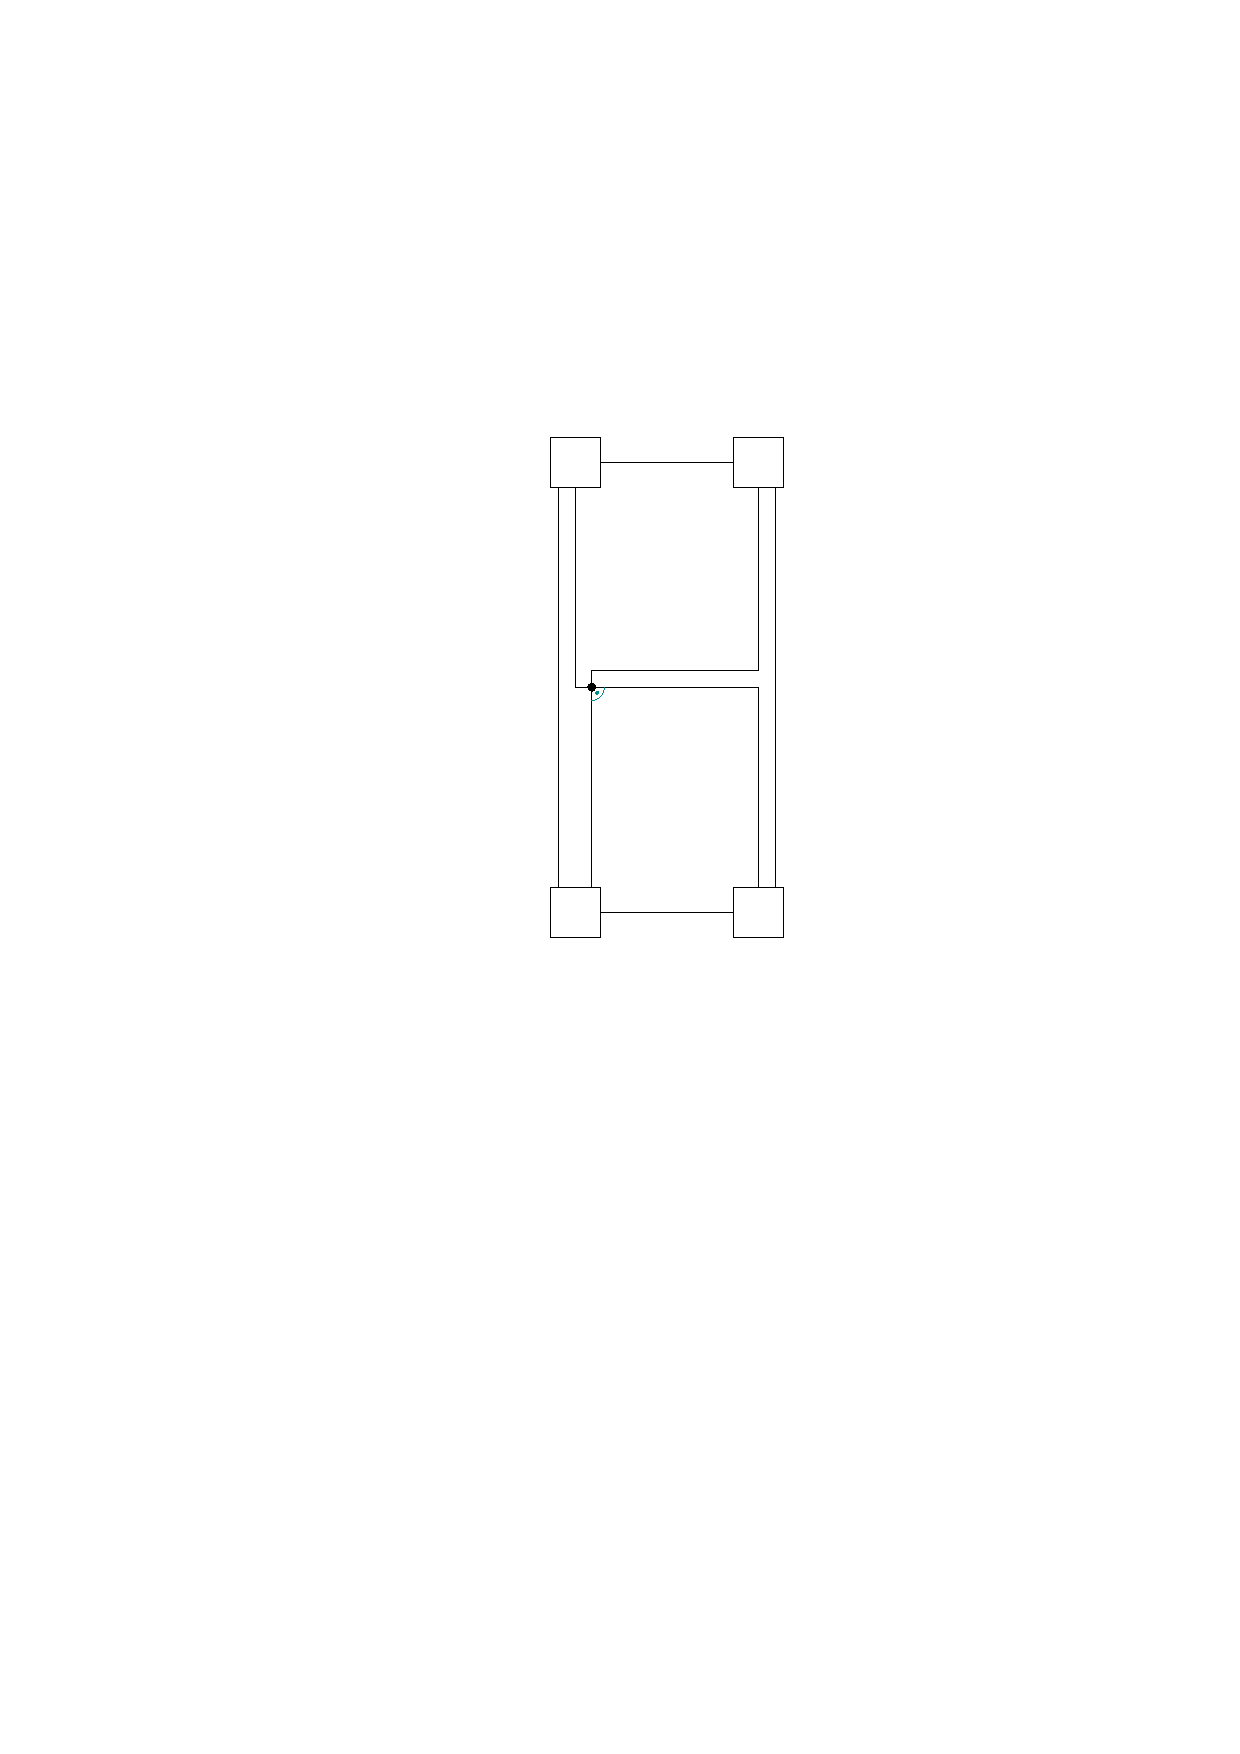
\includegraphics[width=0.5\linewidth,page=1]{includegraphics/new_model_hourglass.pdf}
		\caption{Orthogonal}\label{im:new_model_orthogonal}
	\end{subfigure}
	\begin{subfigure}{0.3\textwidth}
		\centering
		\includegraphics[width=0.5\linewidth,page=3]{includegraphics/new_model_hourglass.pdf}
		\caption{SMOG}\label{im:new_model_SMOG}
	\end{subfigure}
	\begin{subfigure}{0.3\textwidth}
		\centering
		\includegraphics[width=0.5\linewidth,page=2]{includegraphics/new_model_hourglass.pdf}
		\caption{Octi arc solution}\label{im:new_model_eighth}
	\end{subfigure}
	\caption{Various illustrations of the hourglass drawing}\label{im:new_model}
\end{figure}
The orthogonal drawing illustrated in Figure \ref{im:new_model_orthogonal} inherits Kandinsky bends resulting in an edge complexity of $3$. The degree of the graph values 3, so there are three connections per port possible (granularity of the fine grid). Therefore, this drawing is consistent with the Kandinsky model.\\
The SMOG representation in Figure \ref{im:new_model_SMOG} inherits a decrease in the edge complexity by $1$ but the crossing is not illustrated in a visibly clear way. Introducing eighth circular arcs, or \textit{octi arcs}, we could find a compromise between the edge complexity and the visible clear crossing (Figure \ref{im:new_model_eighth}). Note that orthogonality of the crossing is illustrated with a 45\degree~turn compared to the crossing of Figure \ref{im:new_model_orthogonal}.
\subsubsection{Examining the octi arcs}
Using the octi arcs seems to be rather flexible. An octi arc implies a 45\degree~turn in the drawing which is crucial for a smooth representation of diagonally shaped crossings in a drawing.
\begin{figure}[H]
	\centering
	\begin{subfigure}{0.4\textwidth}
		\centering
		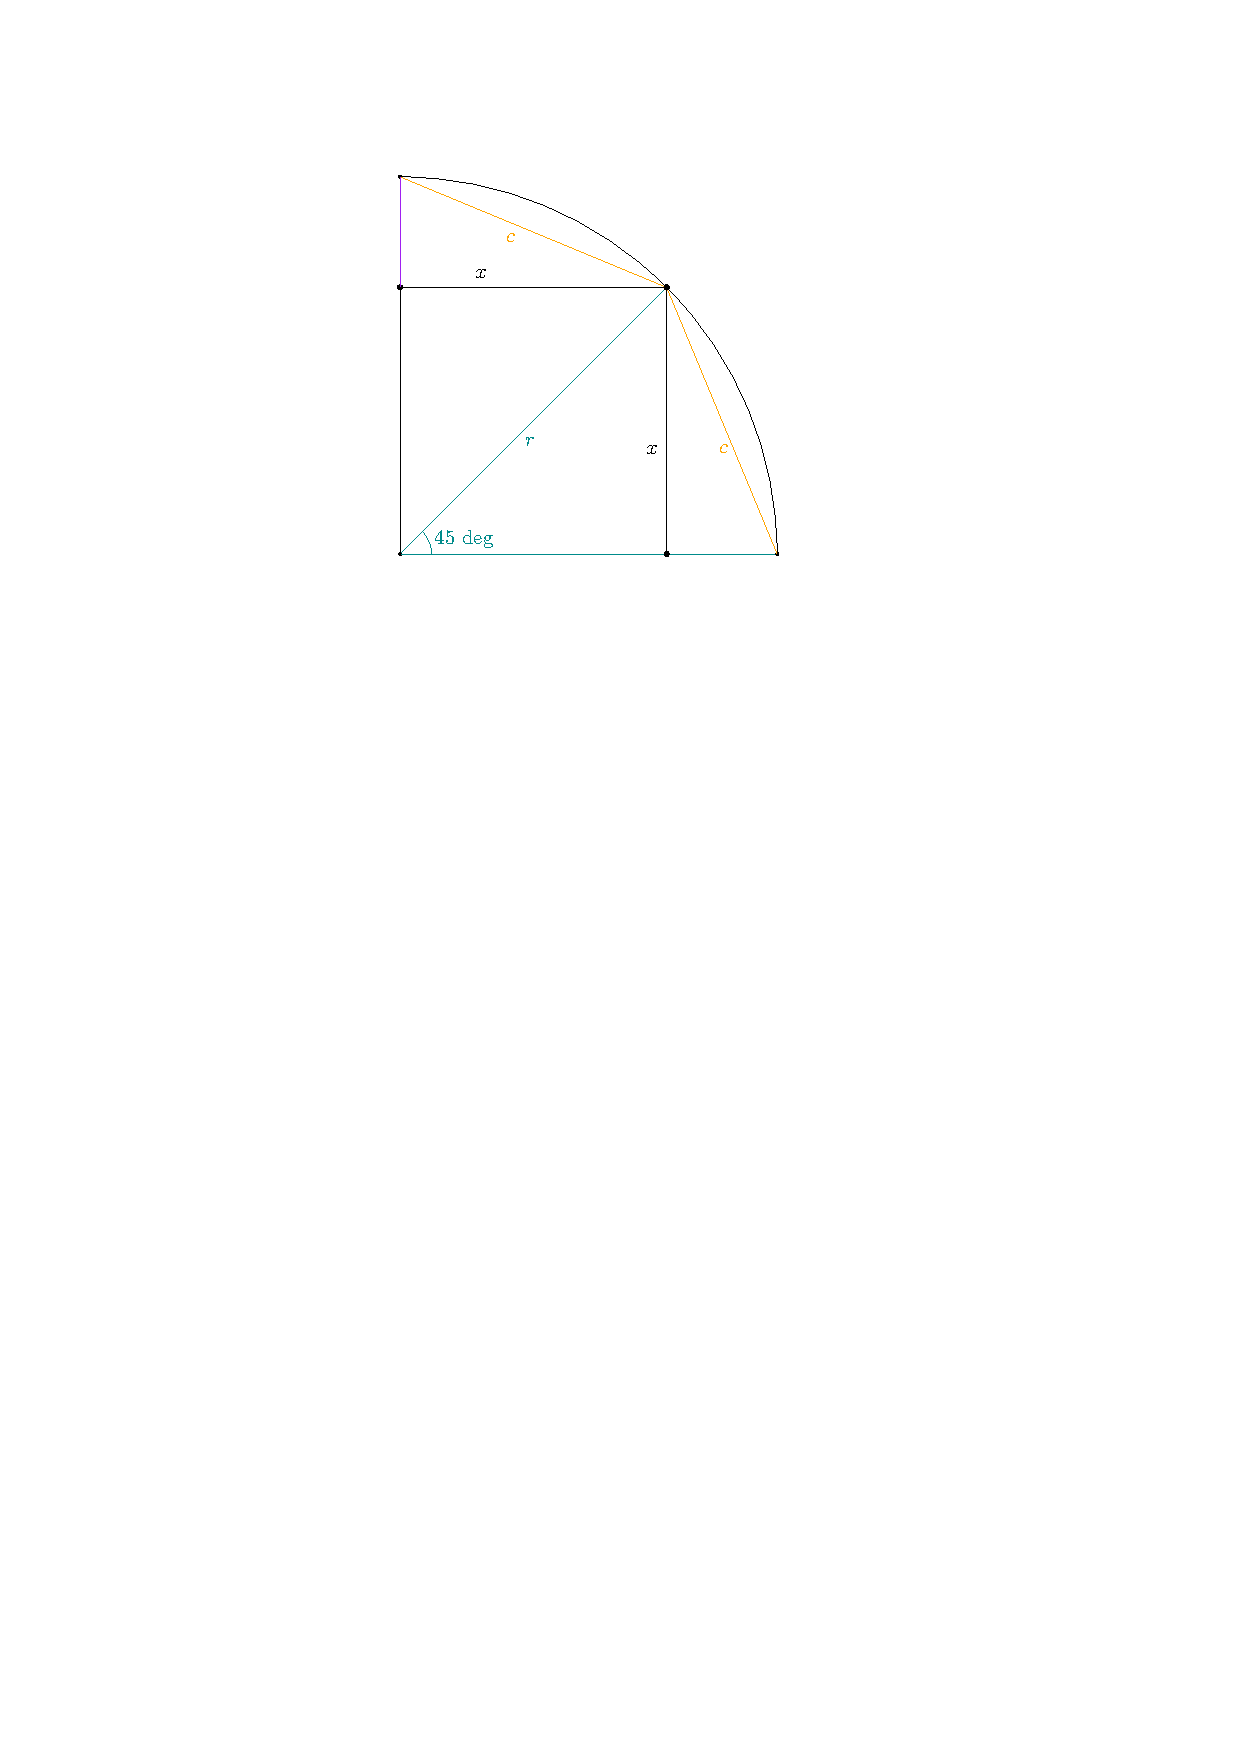
\includegraphics[width=0.7\linewidth,page=1]{includegraphics/new_model_eighth_prop.pdf}
		\caption{Construction}\label{im:exam_eighth_arcs_con}
	\end{subfigure}
	\begin{subfigure}{0.4\textwidth}
		\centering
		\includegraphics[page=2]{includegraphics/new_model_eighth_prop.pdf}
		\caption{In Detail}\label{im:exam_eighth_arcs_detail}
	\end{subfigure}
	\caption{Examination of octi arcs}\label{im:exam_eighth_arcs}
\end{figure}
%\TODO{Schöne Farben raussuchen über \hyperref{www.palleton.com}{}{}{hier}}
Due to trigonometry, the length of several edges can be calculated in dependence of $r$:
\begin{align}
2x^2 &= r^2\\
\Leftrightarrow x &= \frac{r}{\sqrt{2}}
\end{align}
Furthermore, for the distance between the endpoints of an octi arc:
\begin{align}
c^2 &= (r-x)^2 + x^2\\
&= r^2 - 2xr + 2x^2\\
&= r^2 - 2\frac{r}{\sqrt{2}}\cdot r + r^2\\
&= 2r^2 - \sqrt{2}r ^2\\
\Leftrightarrow c &= \left(\sqrt{2-\sqrt{2}}\right)r\\
&\approx 0.7654\cdot r
\end{align}
\subsubsection{Saving Space}
In the previous section, we saw some approaches to effectively save space, either by postprocessing a SMOG or by substituting circular arcs with an adequate alternative. In this section, we will examine whether octi arcs are suitable as a substitution alternative. The smooth 90\degree~bend is achieved by using two octi arcs with different radii and a diagonal segment for flexibility. As we already saw, in order to reach a height of the radius $r$, an octi arc without any further ado reaches a width of $(\sqrt{2}-1)r$. So the sole octi arc is still taking $\Rho(r)$ width. What will happen, if we add another octi arc with a diagonal segment in order to maintain a smooth drawing? The question arises whether we were able to save space. The answer will be - a little bit, but not quite enough in the long run.
\begin{figure}[H]
	\centering
	\begin{subfigure}{0.33\textwidth}
		\centering
		\includegraphics[width=0.7\linewidth,page=3]{includegraphics/cSMOG_arcs.pdf}
	\end{subfigure}
	\begin{subfigure}{0.33\textwidth}
		\centering
		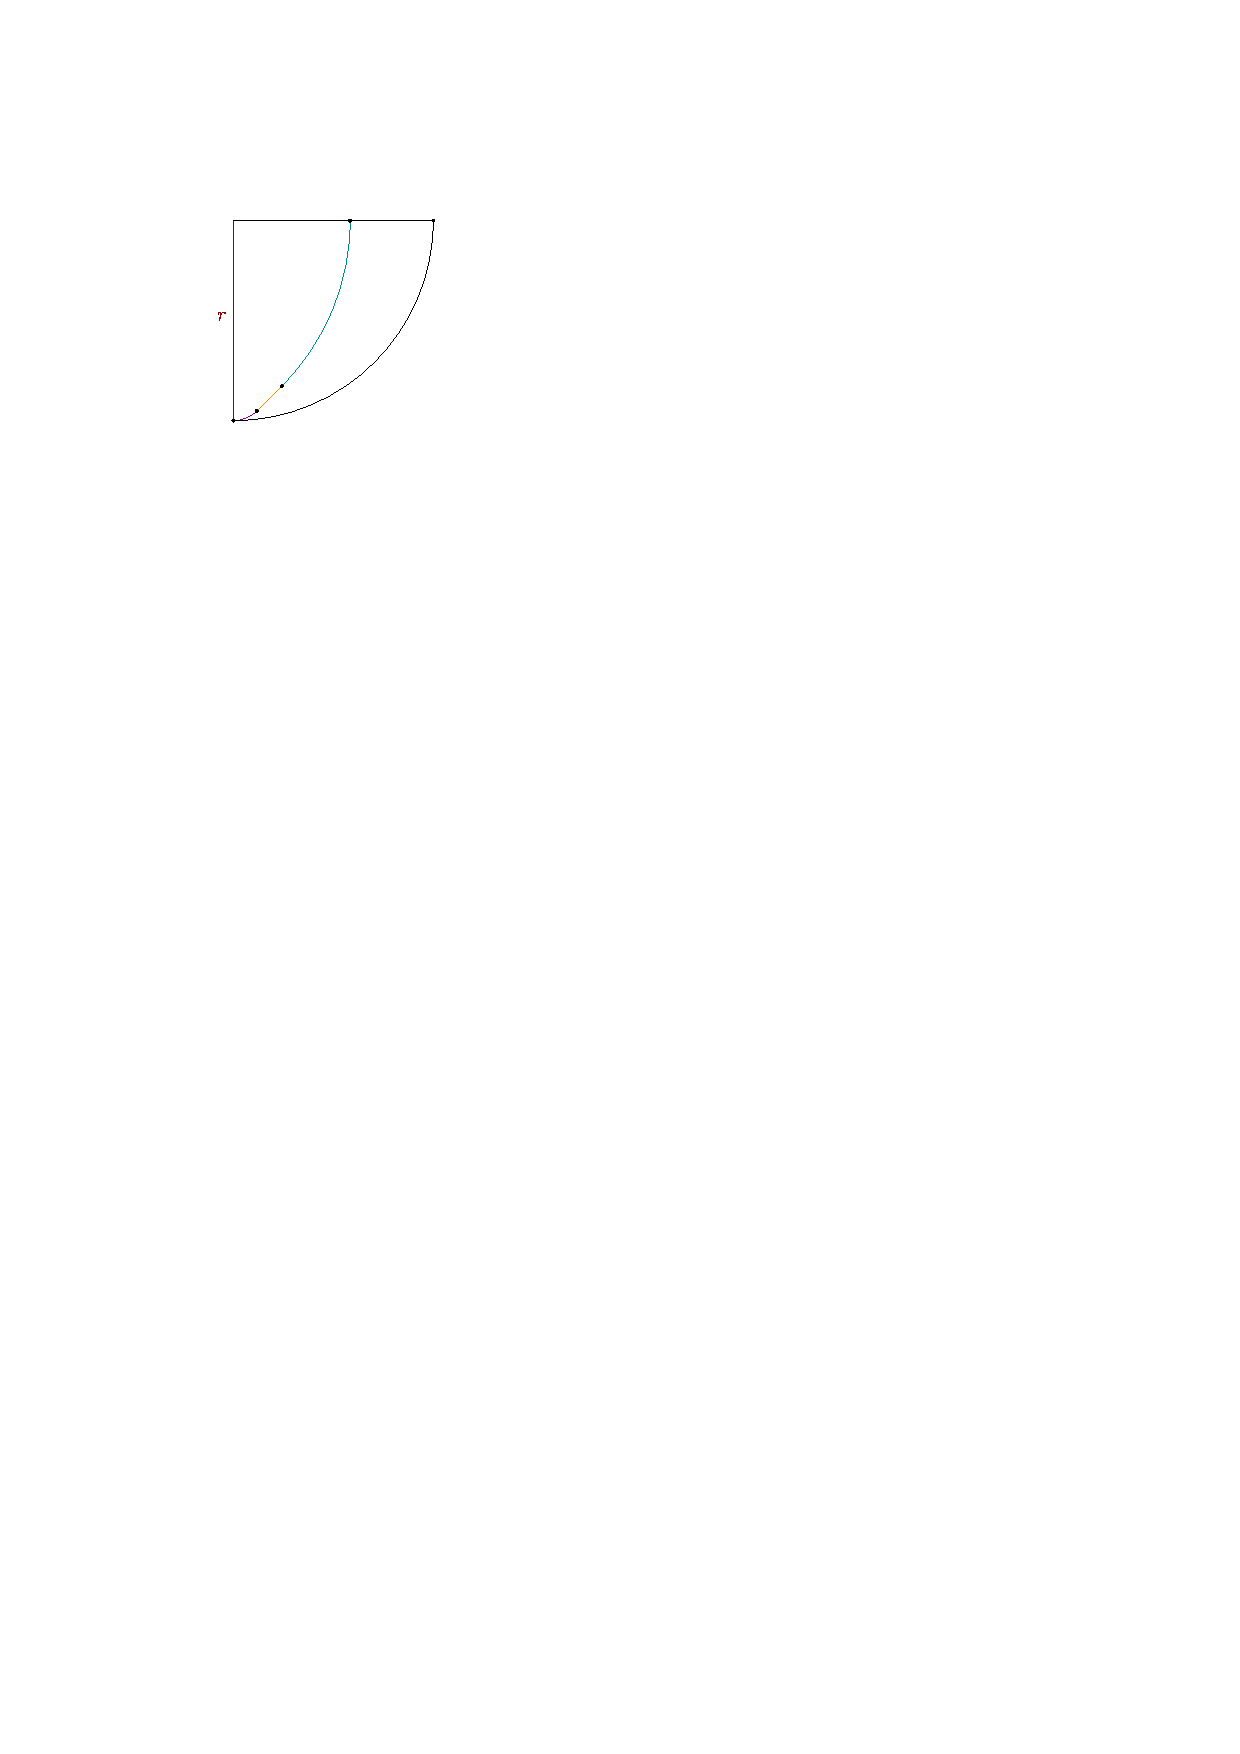
\includegraphics[width=0.7\linewidth,page=1]{includegraphics/cSMOG_arcs.pdf}
	\end{subfigure}\begin{subfigure}{0.33\textwidth}
		\centering
		\includegraphics[width=0.7\linewidth,page=2]{includegraphics/cSMOG_arcs.pdf}
	\end{subfigure}
	\caption{Various ratios of the combination of octi arcs and diagonal segments}
\end{figure}
Introducting a small octi arc to begin with seems to be consistent with the idea of smooth drawings as the resulting bend will be 45\degree~on both sides, resulting in differentiable curves. However, we will see that the width of the suggested combination of segments gets greater as the small first octi arc gets introduced. One one hand, we will save width because the second, big octi arc has less height to overcome, but on the other hand we gain width with the small octi arc getting wider. Let $r$ be the original height to manage, $r'$ the height, the octi arc has to manage together with a small octi arc at the beginning.
\begin{figure}[H]
	\centering
	\begin{subfigure}{0.4\textwidth}
		\centering
		\includegraphics[width=0.7\linewidth,page=5]{includegraphics/cSMOG_arcs.pdf}
	\end{subfigure}
	\caption{Illustration of the combination of octi arcs}\label{im:cSMOG}
\end{figure}
Without loss of generality, we will examine the properties without a diagonal segment. In figure \ref{im:cSMOG}, $r$ describes the height and the original radius of the circular ars. $x$ describes the width gained by two octi arcs.
\begin{align}
r &= \frac{\sqrt{2}-1}{\sqrt{2}}r_1 + \frac{1}{\sqrt{2}}r_2\label{eq:side_comb}&&r_1,r_2 \in (0,r)\\
x &= \frac{1}{\sqrt{2}}r_1 + \frac{\sqrt{2}-1}{\sqrt{2}}r_2\label{eq:main_comb}
\end{align}
From equation \ref{eq:side_comb} we get the following dependency, which is used for equation \ref{eq:main_comb}:
\begin{align*}
&&	r_1 &= \sqrt{2}r - \left(\sqrt{2}-1\right)r_2 &&\\
\Rightarrow &&	x &= \left(\sqrt{2}-1\right)r+2r_2 &&\in \Theta(r)
\end{align*}
Actually we could save some space. With the following radii for the octi arcs we can save half the length of the original radius.
\begin{align}
r_1 := \frac{\sqrt{2}+1}{6}r, r_2:=\frac{1}{6}r &&\Rightarrow x = \frac{1}{2}r
\end{align}
Unforunately, substituting the circular arcs with the mentioned combination in the orthogonal drawing will still take $\Rho(n^2)\times\Rho(n)$ area in the worst case.